\chapter{Die Regionen der heimlichen Lande}


    \begin{figure*}[t]
		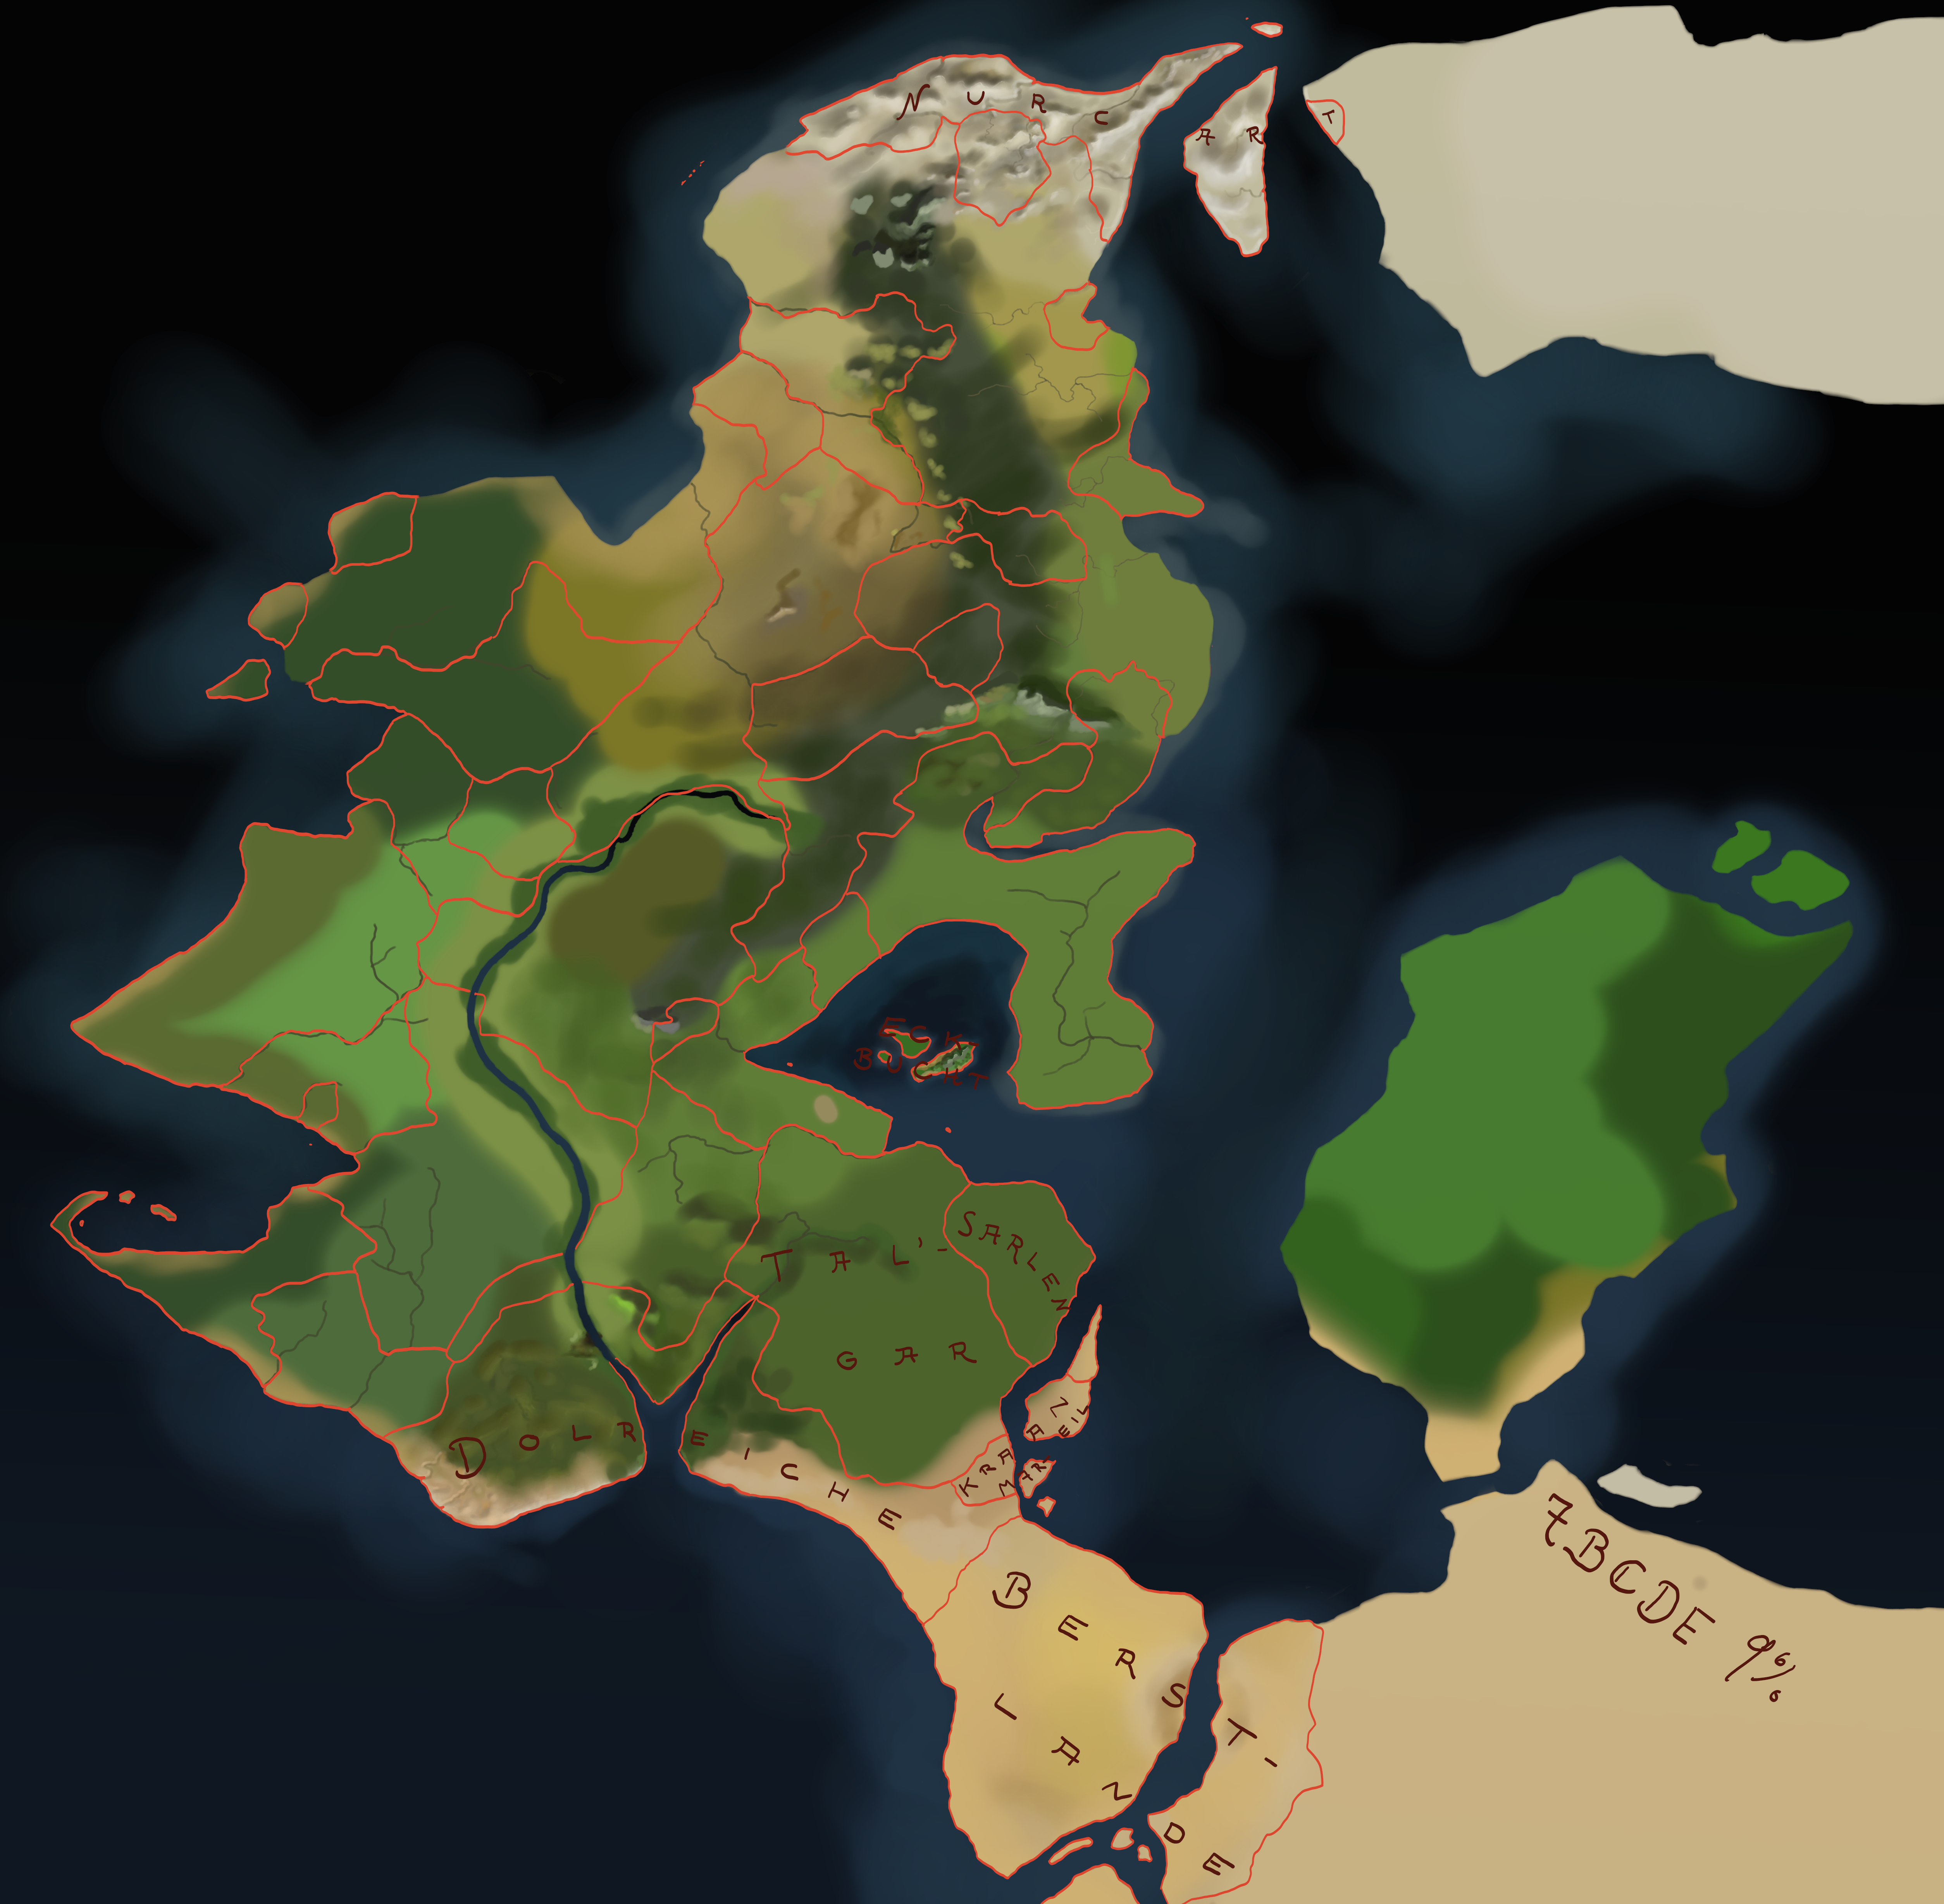
\includegraphics[width=\textwidth]{Pictures/Karte.png}
		\caption{Heimliche Lande}
        \label{fig:Heimliche_Lande}
    \end{figure*}
    
\section*{Aharsh \\ \textit{Einhorndünen}}
Eine ewige karge Ebene, bestückt mit felsigen Zähnen kalten Nächten und wenig Grün. Das rohe, riesige Gebiet im Herz der heimlichen Lande reicht von der Nahrt bis zu den Nordtiken und ist somit auch die längste \textit{regulierte} Region des Kontinents. Wobei reguliert jedoch nicht eine staatliche Verwaltung darstellt, sondern viel ehr die kulture Kategorisierung vieler hunderter Ghulstämme die über die Schluchttiefen verteilt sind, und mit eigenen Kodexen ihre Laargs (Machtgebiete) verwalten. Ohne Frage der bekannteste Stamm ist der Valc Nahk (\textit{Reiterstamm}). Das Bild der Einhörner reitenden Valc-Dorks wurde weit über die Grenzen Aharshs getragen, und sicherlich schon in vielen Malereien niedergefasst. Doch haben auch die Mrotsbauer des Ne'ekl Nahk einen präsenten Namen. Jeder zwei Mrot dieses Jahrzehnts wurde in den Händen dieser fleißigen Orks hoch oben in Ark-Arlsh entworfen, gebaut und eingeweiht. Seine es die rasanten Ratssters oder die großen Voolks, sie alle tragen die pinke Sonne der Nordtikenorks.

\section*{Amerod \\ \textit{Küste des Freiheit}}
Die Abgeschiedenen Füstentümer Amerods, schlossen sich vor 132 Jahren unter dem Banner des weißen Reißadlers zusammen. All ihr fruchtbares, verstreut besiedeltes Land unterstellten sie dem Rat der Türme in der neuen Zentralstadt Kahltenheim. Ein jedes Fürstentum erhielt proportional zu ihrer Fläche Sitze in ihm. So entsendet die Insel Chaltenhoch einen Abgesandten wärend das Fürstentum Schobersten ganze fünf Sitze inne hat. Die Abgesandten sind gewählten Repräsentanten der Menschen der Fürstentümer. Weder die Orks, Wareguards, noch die Vampire des Landes erhalten eine Möglichkeit über das Land zu entscheiden. Im Verhältniss zu den Menschen machen diese Minderheiten auch gerade mal 15\% der Bevölkerung aus. Während die Wareguards die verlassenen Höhlen des vergangenen alten Howlerimperiums im Südosten der Nation bewohnen, finden sich die Vampire im feuchteren Landesinneren, wo sie fröhlich jagen und regelmässig in Konflikte mit der menschlichen Bevölkerung geraten. Die Orks Amerods leben gemeinsam mit dem Mensch verteilt über das fruchtbaren, weite, windige Land. Die Küstenstädte Fuchtlig, Zeign und Trost sammeln die neben der Zentralstadt die meiste Bevölkerung. Ihre Häfen sind wichtige Anlegepunkte für Seefahrer und bieten den wohl besten Bierschaum des gesamten Kontinents. Von ihnen aus führt ein spärliche Netz als verschwommenden Straßen über das lose besiedelte Land. Die unregelmäßig verteilten Dörflein, sind schon von Weiten an den Drachentürmen zu erkennen. Sie verbleiben noch aus der Zeit des Feuerhimmels, als die Drachen der Aschfarbe die Neuzyklen im Süden verbracht haben und auf dem Rückweg sich mit den Winden über Amerod hinweg treiben ließen, wurde als Verteidigung gegen die regelmäßigen Dorfbrande je einer dieser Schleuder bestückten Steintürme errichtet um, wenigsten eine potentielle Gefahr darzustellen. Aus dieser Zeit stammen viele Mythen von mutigen Schützen und sterbenden Drachen.

\section*{Berstlande \\ \textit{Ewiger Stempel}}
Die kargen und vor allem heißen Berstlande markieren den südlichsten Teil der heimlichen Welt. Als einzige Region liegen diese weiten Wüsten in der “hellen Südzone”, also der Zone, die über das gesamte Jahr durchgehend im Licht Veralas liegt. Die sanften, ebenen, weiten Sandgebiete werden gespickt durch die scharfen kanten riesiger Felsbrocken, in deren mächtigen Schatten die Ruinen der alten Welt liegen. Diese Lande waren einst das Zentrum des weißen Reiches gewesen. Heute überbleiben neben verlassenen Ruinen, kleineren Kulten, der Stadt Resaîen und viele Tempel der Alten lediglich die Alten selber als Erinnerung an einen mächtige Vergangenheit.

Die in Tempel lebenden Alten, werden häufig bewacht durch Wareguards und halten sich teilweise Wiedergänger als Diener. Zudem durchstreifen Drachen die weiten Lande und vor allem die fruchtbaren Küstenbereich rund um den sauberen Schnitt auf der Suche nach Nahrung. Zu ihren Opfer zählen neben den normadisch lebenden Howlern teilweise Einhörner oder Sûrhörner (also gestachelte Minotauren). Wo der Nordwesten des Landes fast keine lebende Seele offen zeigt, ist der Südosten dank des sauberen Schnitts teilweise sogar grün. Wo der Schnitt im Süden breiter wird umläuft er die vier Inseln. Gasy, Jurr und Vian sind kleine Inseln bevölkert durch Phoenixe und Silberaffen. H’jer hingegen ist deutlich größer und felsiger. dieses heiße braun-grüne Haufen Erde wird durch die Ungeehrten bevölkert. Eine Gemeinschaft von Vampiren, Sûrhörnern und Silberaffen, mit gemischten Absichten. Mal handeln sie über Seewege mit dem Rest des Kontinents, mal stürmen sie deren Festen und plündern deren Dörfer.

Blickt man nun den sauberen Schnitt hoch nach Norden, so findet man im Osten die riesige Stadt Resaîen. Das Grabgänger- und Sûrhörnervolk wird durch ein Altenrat beherrscht und verehrt die alte Ordnung.

\section*{Dolreich \\ \textit{Drei Kronen Reich}}
Das Dolreich vereinigt die ehemaligen drei Reiche Dermisch, Ohllande und Leichsaal unter der Führung des Hauses Marl.  Im Osten erreicht das dürre Land sogar für ein kurzes Stück das L’armeer. Die primär menschliche und skrivische Bevölkerung bevölkert die Dolbucht sowohl die Nahrt als auch die Var hoch. Vereinzelt leben hier jedoch ebenso Howler, Spheroma und einige Vampire in abgelegenen Dörfern und Vereinigungen.

Das Dolreich bietet eine breite Varianz an Vegetation: Der steinige und hügelige Westen, das Pflanzen freundliche, grün-braune Zentrum und der karge, sandige Osten. Die drei ehemaligen Hauptstädte der Vorreiche bilden heute noch die Hauptknotenpunkte der Macht und des Handels:
\begin{itemize}
    \item Dermatan liegt auf der Westseite der Nahrt. Dieses Metropole ist Hauptstadt des Dolreichs, primärer Hafen des Wasserhandels und ein Kunststück der frühsiedlerischen Bauweise. Um den erhöhten und befestigten Stadtkern schlängeln sich die Spiralarme der Straßen, bestückt mit den Gebäuden der niederen Schicht. Die “Brücke” ragt vom Kern bis zur Naht und sichert somit einen direkten Zugang der hohen Herren zum Geld bringenden Wasser.
    \item Meralith ist eine wahrhaft bezaubernde Stadt. Die von starken Stadtmauern eingefasste Stadt liegt ruhig in den bebauten Hügeln des Ohllandes. Das als Bauernsiedlung gewachsene Dörfchen entwickelte sich in den dunklen Jahren zu einer Zufluchtsstelle der einfachen Bevölkerung. In den Leichenkriegen starben Großteile der Bevölkerung, so dass bis heute das schwarze Viertel verlassen im Norden der Stadt ruht.
\end{itemize}

\section*{Kraan Mareil \\ \textit{Felseninseln}}

Als die “Blutwurzeln” oder die “Höhen des kargen Tods” werden die Kraan Mareil in Sagen und Mythen umschrieben. Seit einigen tausend Jahren ist die von steinigen Höhen und trockenen Tiefen dominierte Küstenregion mit ihren Inseln Gebiet der gefürchteten Saan Mareil - den Piraten der Felsen. Von hier aus operiert die vampirische Seemacht und plant ihre nächsten Raubzüge. Die natürlichen Felsfronten bieten den leichtfüßigen Vampiren ein nahezu uneinnehmbares Territorium voller Möglichkeiten ihre perversen Folterfantasien freien Lauf zu lassen. Als Untergebene Rasse leben viele Harpyien vor allem in den Haupthäfen, um ihren übergeordneten Meistern nicht nur in Seeschlachten zur Seite zu stehen. Diese zentralen Häfen liegen sich im schwarzen Dreieck gegenüber:
\begin{itemize}
    \item Rhuus Fareii auf dem Festland ist der größte Hafen der Flotte. Die Tunnel- und Hängebrückensysteme ziehen sich tief durch das Inland und ermöglichen es so den Bewohnern schnell durch das unwegsame Gelände zu kommen.
    \item Merellee Fareii ist auf der mittleren der drei Kraan Inseln. Hier lebt vorallem der niedere Stand der Vampire in simlen Höhlen und geflochtenen Holzglocken. Die meisten Schiffe der Flotte werden in den Werten Merellee Fareiis errichtet.
    \item Saan Fareii ist der Hafen der schmutzigsten und erfolgreichesten Adeligen im Volk. Hier landen die besten Schätze und saftigsten Gefangene. Als einzigster Hafen in Kraan Mareil ist es den Harpyien hier untersagt den rauen Boden mit ihren Füßen zu beschmutzen. Verächtlich nennen sie diesen Hafen bloß “die Weiße” um die übertriebene Reinheit auszudrücken.
\end{itemize}

\section*{Sarlen \\ \textit{Schlammtäle}}

Die freien Regionen im Süden der Eckbucht werden unter dem Namen Sarlen zusammengefasst. Das schwüle, matschige Land ist unter der Kontrolle der Natur und ermöglicht es unabhängigen Sirenerotten, kleineren Minotauren Dörfern, Krograts und auch einigen Harpyien ein Leben ohne den Zwang durch Herrschaftssysteme. Jedoch bringt diese Freiheit auch Gefahren mit sich: Nicht selten kommen Jagdgruppen der Ghule hoch in den Nordosten um sich einen Rang und Namen zu verdienen. Jedoch ist auch schon das Leben ohne eine externe Gefahr hart, da ein jeder hier überleben möchte und im Zweifelsfall bereit ist über Leichen zu gehen.

\section*{Nietküste \\ \textit{Zahnrad der Zeit}}

Kaum ein Stück Land wurde so von der Flut der Skriva gezeichnet wie das windige Küstenstück zu Fuße der Schuppentiken. Gerade mal 120 Jahre nachdem die Menschen und Minotauren in den windgeschützten Neuecktälern Fuß gefasst hatten, wurden sie mit den fliehenden Skrivas in jeder Hinsicht überfordert. Egal wie gut die Ernte war, egal wie viel Land sie bieten konnten, es gab stets ein Maul zu viel und ein paar Beine zu viel. Dies war der Zeitpunkt, an dem man begann die Häuser an Felswenden in die Höhe zuziehen, das berühmt Eckbrüh an zu richten und die wiederlichen Neilfrösche auf die Speiselisten zu setzen. Selbst als die Skrivaflut abriss, und die Felder erweitert wurden, überdauerten die neu gefundenen Traditionen. Sie wurden ausgearbeitet und dank den schlauen Konzepten der Arlt-Mauer-Gemeinschaft begann der Überschwall an Fellfreunden plötzlich den Wohlstand der kleinen Nation zu beflügeln. Nicht nur sprudelten die Minearalien wie Wasser aus der Erde, sondern wurden von den Händen innovativ denkender Menschen und Skriva zu Skailen verarbeitet. Diese kunstvollen, mechanischen Konstruktionen basierten nicht auf Spiritkräften wie Mrots, sondern fanden ihren Ursprung in Mechanik und Chemischen Prozesse, was sie unabhängig von Feldverteilungen überall funktionieren ließ. Unter dem Banner des Fortschrittes und der Kooperation bildeten sich die Banken wie die \textit{Krey \& Wayne Kastbank}, Handelsgemeinschaften und die ersten Multikontinentalen Schifffahrtslinien.

\section*{Nurcart \\ \textit{Kalter Stachelpanzer}}

Nurcart ist ein kaltes erbarmungsloses Land. Es zieht sich entlang der Küste und über die schwarze Insel bis rüber über den zweiten Graben. Nurcarts Landschaft ist große Teile des Jahres mit Schnee bedeckt und stellt mit seinen schwarzen Gesteinszähnen ein kontrastreiches Bild dar. Einzelne Nadelbäume sind die kostbaren Holzquellen welche einzuteilt gewusst werden sollten.

Nurcart ist weder ein Staat noch ein Bund, sondern lediglich ein Begriff für die vielen Kreise der Cartregion. In den Kreisen leben Draekolins, Silberaffen, Minotauren, Daemonen und einige Rudel von Ghulen. Die Kreise handeln viel übers Wasser und so ist es kein Wunder, dass die größten Kreise am ersten und zweiten Graben liegen. So sind der ganz im Osten liegende K'lae Tur (Kreis der Träne), die Kreise K'lae Serk (Kreis des Eindrucks) und K'lae Kha (Kreis der Fruchtbarkeit) auf der schwarzen Insel zwar nicht auf dem Heimatkontinent, dennoch laufen zwei Drittel aller Handelsrouten des Osthandels durch die Tore dieser drei Kreise.

Jede 281ste Flut treffen sich die Kreisanführer in den 5 Region (Gaashs) um sich zu beraten. Seien es lokale Konflikte, neue Regeln, Handelspläne oder ein erneuter Marsch nach Süden um die Wildnis fern zu halten. Beim Tod eines Anführers stellt eine der 7 Gilden (Gufuars) den nächsten Anführer. Dieses Recht rotiert seit jeher durch die sieben Gufuars.

\section*{Tal’Gar \\ \textit{Invasorenreich}}

Seit Mumrak Gar 26 n.Z. als Anführer des Tal-Klans den Stahl-Klan in die Knie zwang expandierte der Klan in alle Himmelsrichtungen. Sie schlugen die Sirenen im Norden, die Minotauren an der Eckbucht, die Menschen im Westen, die Skriva im Süden und sogar die Vampire im Osten. Heute erstreckt sich das Reich der Tal’Gar zwischen dem Dolreich im Süden und der Eckbucht im Norden. Das kriegerische Ghulvolk lebt in verschiedenen Klans, welche alle dem Gar verpflichtet sind. Das heißt aber nicht, das sie wie Verbündete gemeinsam kämpfen würden. Ganz im Gegenteil. Die Rivalitäten der Ghulklans kostet jedes Jahr viele hundert Leben. Lediglich wenn der Gar die Blutfichte ergreift versammelt sich das gesammte Volk auf den Feldern des Krieges um einen neuen Schlag durchzuführen.

Zum Glück der Nachbarn ist der aktuelle Gar Kosh’ma ein recht Gold versessener Dork, welcher sich mit gewinnbringenden Verträgen zufrieden stellen lässt. Es ist jedoch nur eine Frage der Zeit, dass er seinen Platz als Gar gegen den Tod eintauschen wird - und wer der nächste Gar wird ist eine ganz andere Frage…

\section*{Valkheit \\ \textit{Herz der Ehre}}

Feuchte, begrünte Erde die unter den Fußstapfen der durch den Wald jagenden Njarkla freudig aufgeworfen wird. So wird das Land der gläubigen Orden und matschigen Straßen beschrieben. In Wahrheit ist es ehr das Land der giftigen Insekten, der großen Jagerduuns und des fröhlich Besäufnisses. Die großen Kahlteranlagen der neunzehn Orden dienen als Sammelpunkt für Handel, Schwert und Konkurenz, während in den Schatten der Schuppentiken still und heimlich das Imperium der neuen Sonne auf ersteht.
Die grüne Valkheit wird primär von den achtsamen Krograts und den machtgierigen Menschen bevölkert. Während die Schuppenechsen die feuchten Wälder sein eigen nennt, kann man den Menschen gerade im Norden des Landes antreffen. Dort stehen die großen weißen Türme Saxreiks, die Brücken Nynklas und die großen Straßen Lierens. All diese großartigen Bauwerke wurden im letzten Jahrzehnt unter dem großen Ermptus Siltran Norls erbaut, welcher nicht bloß die Infrastruktur des Nordensförderte sondern auch nach und nach einen Keil in Süden getrieben hat. Die Konflikte zwischen den innovativen Konzepten und dem gläubigen Ordenstum spannen sich längst nicht mehr nur auf Briefen und droht den mächtigen Osten der heimlichen Lande in einen Konflikt zu stürzen der sich nicht von alleine schlichten lassen wird.

\section*{Vernen \\ \textit{Das gehörnte Land}}

Kaum ein Land ist so grün, so belebt, so multikulturell der Machtspielball Vernen. Unter der Kontrolle der Nachbarnationen grünt es nun nach nach der Zeit des Westkonflikts wieder auf. Als ehemalige Ostflanke des Deutenreichs wurde es von der Herrschaft der Skrandalen befreit und ist nun Heimat für die verschiedensten Wesen. Die Ansammlungen von Skriva, Menschen, Minotauren und Wareguards die sich gemeinsam in kleinen neu geformten Zivilisationen an ein gemeinsames Feuer zwängen stehen jedoch im direkten Kontrast zu den verbrannten und niedergerissen Großstädten. Die aschebeschichteten Straßen werden noch immer von Leichensuchern begutachtet und von Bettlern überschwämmt. Sie alle haben den Preis der falschen Zeit und des falschen Ortes bezahlen müssen. Sie sehen mit wehmütigen Augen rüber in die letzte stehende Stadt: Maltena. Die junge Stadt spross einst auf der Erde der gläubigen Nunta Stämme - lose Gruppierungen von Minaotauren und Witchghulen. Als sie unter die Finger der Skrandalen fiehlen lernte sie den Bau von stabilen großen Häusern, den Umgang mit modernen Werkzeug und das bändigen der Stachelwölfe. Auch wenn heute die Stachelwölfe in den Straßen fehlen, können noch viele sehr experimentelle Mischbauten aus Stein und Holz gefunden werden, die den Beginn der Stadt markieren.